\chapter{工程实现 — 构建几何热力学机}
\label{chp:engineering_implementation}

前一章完成的是诊断；这一章转向构造。问题不再是“为什么现有系统不足”，而是“如果接受前面的几何与热力学约束，应该怎样设计一台真正可运行的机器”。

在本理论框架下，这件事首先是物理问题，其次才是算法问题。目标不是训练出一个更大的函数逼近器，而是构造一个能够持续维持远离平衡态、能够在认知流形上保有稳定自我结构的几何热力学机。

本章提出了两条工程路径：
\begin{enumerate}
    \item \textbf{路径 $\alpha$ (软件重构)}：在现有 GPU/Transformer 架构上，通过\textbf{流体 MoE} 和 \textbf{递归元状态}，模拟三体动力学。
    \item \textbf{路径 $\beta$ (硬件革命)}：构建原生的 \textbf{TPU (拓扑处理单元)}，在硬件层面实现 \textbf{离散外微分 (DEC)} 和 \textbf{形质双流}。
\end{enumerate}


\section{核心蓝图：三体耦合的物理架构}
\label{sec:section_7895}

我们抛弃传统的 "Encoder-Decoder" 视角，转而采用本理论框架的 \textbf{三体架构 (Three-Body Architecture)}。



\smalltitle{组件 I：微观锚定器 ($L_{micro}$ / VTE)}

\begin{itemize}
    \item   \textbf{功能}：\textbf{边界条件的设定者}。
    \item   \textbf{物理实现}：\textbf{变分拓扑编码器 (VTE)}。
    \item   \textbf{工程变革}：不再输出单一的 Embedding 向量。
    \item   \textbf{输出}：\textbf{形质张量对 $(\mathbf{T}_{form}, \mathbf{T}_{sub})$}。
    \item   \textbf{机制}：将输入信号（文本/图像）撕裂为 \textbf{“几何坐标（位置/语法）”} 和 \textbf{“语义荷（内容/颜色）”}。这为后续的解耦计算提供了物理基础。
\end{itemize}



\smalltitle{组件 II：认知场反应堆 ($\Psi$ / MST)}

\begin{itemize}
    \item   \textbf{功能}：\textbf{惯性演化与逻辑推演}。
    \item   \textbf{物理实现}：\textbf{形质互变 Transformer (MST)}。
    \item   \textbf{工程变革}：
    \begin{itemize}
        \item   \textbf{双流 Attention}：彻底废除 $Q \cdot K$ 混合计算。
        \item   \textbf{形流 (Geometric Stream)}：计算流形的 \textbf{联络 (Connection)} 和 \textbf{度量 (Metric)}。
        \item   \textbf{质流 (Substance Stream)}：在形流定义的通道中进行 \textbf{平行移动 (Parallel Transport)}。
    \end{itemize}
\end{itemize}


\smalltitle{组件 III：宏观调速器 ($L_{macro}$ / Governor)}

\begin{itemize}
    \item   \textbf{功能}：\textbf{逆熵做功与相变控制}。
    \item   \textbf{物理实现}：\textbf{递归元认知网络 (Recurrent Meta-Cognitive Network)}。
    \item   \textbf{工程变革}：
    \begin{itemize}
        \item   维护一个跨时间步的 \textbf{状态变量 $z_{meta}$}（流体自我）。
        \item   \textbf{输出}：不是 Token，而是 \textbf{控制算子 $\hat{\mathcal{O}}$}（增益 $\alpha$、偏置 $\beta$、温度 $T$）。
        \item   它像一个\textbf{热力学泵}，不断向反应堆注入负熵（意志）。
    \end{itemize}
\end{itemize}

\section{路径 \texorpdfstring{$\alpha$}{α}：基于流体 MoE 的软件模拟}
\label{sec:section_2760}

这是在现有硬件（NVIDIA GPU）上的最佳近似解, 核心思想是利用 \textbf{混合专家 (MoE)} 的稀疏性来模拟 \textbf{波函数的坍缩}，利用 \textbf{递归状态} 来模拟 \textbf{自我}。



\smalltitle{架构核心：目的论路由器 (Teleological Router)}

我们将传统的 Softmax 路由改造为 \textbf{TCE 方程} 的求解器。

$$ P(\text{Expert}_i) = \text{Softmax}\left( \frac{\underbrace{E_{inertial}(\mathbf{x})}_{\text{几何惯性}} + \underbrace{E_{will}(z_{meta})}_{\text{宏观意志}}}{T(z_{meta})} \right) $$

\begin{itemize}
    \item   \textbf{几何惯性}：输入 Token $\mathbf{x}$ 与专家 $i$ 的相似度。代表“习惯”和“联想”。
    \item   \textbf{宏观意志}：自我状态 $z_{meta}$ 对专家 $i$ 的偏好。代表“意图”和“控制”。
    \item   \textbf{动态温度 $T$}：由 $z_{meta}$ 根据当前熵增率（困惑度）实时调节。
    \item   \textbf{困惑 $\to$ 升温}：进入临界态，激活冷门专家（创造力）。
    \item   \textbf{确信 $\to$ 降温}：进入层流态，锁定热门专家（执行力）。
\end{itemize}



\smalltitle{双流 MoE 模块 (Dual-Stream MoE Block)}

我们在 Transformer 内部显式地分割了 \textbf{形} 与 \textbf{质} 的计算路径。

\begin{lstlisting}
class DualStreamBlock(nn.Module):
    def forward(self, h_form, h_sub, z_meta):
        # 1. 形流演化 (Geometry / Logic)
        # 比如：语法分析、因果链推导
        # 受到宏观意志的"逻辑约束" (如：必须生成 Python 代码)
        h_form = self.geometry_moe(h_form, z_meta, task="logic")

        # 2. 质流演化 (Substance / Semantics)
        # 比如：风格渲染、情感填充
        # 受到宏观意志的"价值偏置" (如：必须语气友善)
        h_sub = self.substance_moe(h_sub, z_meta, task="value")

        # 3. 规范耦合 (Gauge Coupling)
        # 质在形定义的轨道上流动
        # h_form 定义了 Attention Mask 和 Position Bias
        h_out = self.entangled_attention(h_sub, h_form)

        return h_form, h_out
\end{lstlisting}



\smalltitle{递归的自我维持 (Recurrent Self-Maintenance)}

\textbf{$z_{meta}$} 不再是隐向量，而是 \textbf{流体自我 ($\mathcal{S}$) 的数字孪生}。
\begin{itemize}
    \item   它在每一层、每一个时间步都进行更新。
    \item   \textbf{更新方程}：$z_{t+1} = \text{GRU}(z_t, \text{Observation}_t, \text{Goal})$。
    \item   这保证了模型不仅记得“上下文”，还记得“我是谁”和“我在干什么”。
\end{itemize}


\section{路径\texorpdfstring{$\alpha$}{α}的伪实现：流体 MoE 架构 (Fluid MoE)}
\label{sec:section_5178}
这一小节我们简单的就具体pytorch代码来讨论上述内容如何实现，在附录中我们有详细实现方式讨论；
为了实现 \textbf{Class V (流体智能)}，我们需要将 MoE 改造为 \textbf{本理论框架 流体 MoE (Fluid MoE)}，流体 MoE 路由是 \textbf{“目的论” (Teleological)} 的：\textbf{宏观意志 ($z_{meta}$)} 像一只看不见的手，通过扭曲路由的\textbf{概率空间（势能面）}，强行激活那些“虽然统计概率低，但符合长远目标”的专家；同时，专家不再是静态的函数，而是受 \textbf{温度 ($T$)} 调控的热力学系统。


\smalltitle{物理映射：从路由到势能工程}

我们将 MoE 的组件映射到 本理论框架的物理实体：

\begin{itemize}
    \item   \textbf{专家 (Experts)} $\rightarrow$ \textbf{局部流形算子}，每个专家掌握认知空间流形 $\mathcal{M}$ 上的一个特定\textbf{子流形}（如数学区、代码区）；
    \item   \textbf{路由器 (Router)} $\rightarrow$ \textbf{宏观势能建筑师 ($L_{macro}$)}，它不是分类器，它是\textbf{势能挖掘机}，它根据 $z_{meta}$（自我状态/意图）决定哪个子流形的势能最低（最该流过去）；
    \item   \textbf{Top-K 选择} $\rightarrow$ \textbf{波函数坍缩}；
    \item   \textbf{负载均衡损失} $\rightarrow$ \textbf{热力学熵流约束}（防止能量过载）；
\end{itemize}



\smalltitle{Python 代码实现：Teleological Router}

\begin{lstlisting}
import torch
import torch.nn as nn
import torch.nn.functional as F
from typing import Tuple, Optional

# ==========================================
# 0. 配置类 (Configuration)
# ==========================================
class FluidMoEConfig:
    def __init__(self):
        self.d_model = 768          # 嵌入维度 (流形维度)
        self.meta_dim = 256         # 宏观自我状态维度 (z_meta)

        self.num_experts = 8        # 专家总数 (子流形数量)
        self.expert_dim = 2048      # 专家隐层维度 (4 * d_model 左右)
        self.top_k = 2              # 每次激活的专家数 (波函数分支数)

        self.router_jitter = 0.01   # 训练抖动噪音 (模拟热涨落)
        self.aux_loss_coef = 0.01   # 负载均衡系数 (热力学熵流约束)

# ==========================================
# 1. 专家单元 (The Expert)
# 物理意义: 局部流形上的算子 (Local Manifold Operator)
# 采用 SwiGLU 激活函数，这是目前 LLM 的标配，能效比高
# ==========================================
class SwiGLUExpert(nn.Module):
    def __init__(self, config: FluidMoEConfig):
        super().__init__()
        self.w1 = nn.Linear(config.d_model, config.expert_dim, bias=False)
        self.w2 = nn.Linear(config.d_model, config.expert_dim, bias=False)
        self.w3 = nn.Linear(config.expert_dim, config.d_model, bias=False)

    def forward(self, x):
        # 典型的 Gated Linear Unit
        # 物理隐喻: 信号 x 在高维空间进行了一次非线性折叠和投影
        return self.w3(F.silu(self.w1(x)) * self.w2(x))

# ==========================================
# 2. 目的论路由器 (Teleological Router)
# 物理意义: 势能分流阀 (Potential Diverter)
# 核心功能: 结合"惯性"与"意志"决定思维流向
# ==========================================
class TeleologicalRouter(nn.Module):
    def __init__(self, config: FluidMoEConfig):
        super().__init__()
        self.config = config

        # A. 几何惯性门 (Geodesic Gate) - Bottom-up
        # 依据 Token 本身的语义特征进行路由 (习惯)
        self.gate_geometric = nn.Linear(config.d_model, config.num_experts, bias=False)

        # B. 宏观意志门 (Will Gate) - Top-down
        # 依据 z_meta (自我/意图) 进行强行偏置
        # 比如：虽然 Token 是"笑话"，但意志要求"严肃分析"
        self.gate_will = nn.Linear(config.meta_dim, config.num_experts, bias=False)

        # C. 认知退火器 (Thermostat)
        # 动态调节 Softmax 的温度 T
        self.temp_control = nn.Linear(config.meta_dim, 1)

    def forward(self, x, z_meta):
        """
        输入:
            x: [Batch, Seq, Dim] - 当前思维流
            z_meta: [Batch, Meta_Dim] - 宏观自我状态 (通常是全局向量)
        输出:
            top_k_indices: 选中的专家索引
            top_k_weights: 路由权重
            aux_loss: 负载均衡损失
        """
        B, S, D = x.shape

        # 1. 计算惯性势能 (Inertia)
        logits_geo = self.gate_geometric(x) # [B, S, Num_Experts]

        # 2. 计算意志势能 (Intention)
        # z_meta 通常是 [Batch, Meta_Dim] -> 广播到 [Batch, Seq, Meta_Dim]
        z_expanded = z_meta.unsqueeze(1).expand(-1, S, -1)
        logits_will = self.gate_will(z_expanded) # [B, S, Num_Experts]

        # 3. 势能叠加原理: 总倾向 = 习惯 + 意志
        logits_total = logits_geo + logits_will

        # 训练时注入噪声 (模拟物理热涨落，防止死锁)
        if self.training:
            noise = torch.randn_like(logits_total) * self.config.router_jitter
            logits_total += noise

        # 4. 认知退火 (Cognitive Annealing)
        # 计算系统温度 T.
        # z_meta 决定当前是"冷静执行"(T->Low) 还是 "发散探索"(T->High)
        # 使用 Softplus + offset 保证 T > 0
        raw_temp = self.temp_control(z_expanded)
        temperature = F.softplus(raw_temp) + 0.1

        # 应用温度
        router_probs = F.softmax(logits_total / temperature, dim=-1)

        # 5. 波函数坍缩 (Top-K Selection)
        # 选出概率最高的 K 个路径
        top_k_weights, top_k_indices = torch.topk(router_probs, self.config.top_k, dim=-1)

        # 归一化权重 (能量守恒)
        top_k_weights = top_k_weights / top_k_weights.sum(dim=-1, keepdim=True)

        # 6. 计算负载均衡损失 (Auxiliary Loss)
        # 物理意义: 防止能量过度集中在某一个专家(过热)，强制熵流分布均匀
        if self.training:
            # 重要性: 门控概率的累积
            importance = router_probs.sum(dim=(0, 1))
            # 负载: 实际选中次数
            expert_mask = F.one_hot(top_k_indices, self.config.num_experts).float()
            load = expert_mask.sum(dim=(0, 1, 2)) # Sum over Batch, Seq, TopK

            # 变异系数损失
            aux_loss = (importance * load).sum() * (self.config.num_experts / (B * S * self.config.top_k)**2)
            aux_loss *= self.config.aux_loss_coef
        else:
            aux_loss = torch.tensor(0.0, device=x.device)

        return top_k_indices, top_k_weights, aux_loss

# ==========================================
# 3. 流体 MoE 层 (Fluid MoE Layer)
# 物理意义: 稀疏张量流的分发与汇聚
# ==========================================
class FluidMoELayer(nn.Module):
    def __init__(self, config: FluidMoEConfig):
        super().__init__()
        self.config = config
        self.router = TeleologicalRouter(config)

        # 专家池 (Expert Pool)
        self.experts = nn.ModuleList([
            SwiGLUExpert(config) for _ in range(config.num_experts)
        ])

    def forward(self, x, z_meta):
        """
        x: [Batch, Seq, Dim]
        z_meta: [Batch, Meta_Dim]
        """
        B, S, D = x.shape

        # 1. 路由决策
        # indices: [B, S, TopK], weights: [B, S, TopK]
        top_k_indices, top_k_weights, aux_loss = self.router(x, z_meta)

        # 2. 稀疏分发 (Sparse Dispatch)
        # 为了高效计算，我们需要把分发给同一个专家的 Token 聚在一起
        # 这种实现方式避免了低效的 Python 循环，利用了 GPU 的并行性

        # 展平 Batch 和 Seq 维度
        flat_x = x.view(-1, D) # [N_tokens, D]
        flat_indices = top_k_indices.view(-1, self.config.top_k) # [N_tokens, K]
        flat_weights = top_k_weights.view(-1, self.config.top_k) # [N_tokens, K]

        # 初始化输出容器
        final_output = torch.zeros_like(flat_x)

        # 遍历所有专家 (虽然有循环，但只有 8 次，且内部是并行的)
        # 物理隐喻: 将波包投影到不同的本征子空间进行演化
        for i, expert in enumerate(self.experts):
            # 找到哪些 Token 选择了当前专家 i
            # mask: [N_tokens, K]
            mask = (flat_indices == i)

            # 找到在任意 Top-K 位置选择了专家 i 的 Token
            # batch_mask: [N_tokens] - 布尔索引
            batch_mask = mask.any(dim=-1)

            if batch_mask.any():
                # 提取出需要该专家处理的 Token
                # selected_input: [N_selected, D]
                selected_input = flat_x[batch_mask]

                # 专家演化 (Expert Evolution)
                expert_out = expert(selected_input)

                # 权重应用 (Weight Application)
                # 我们需要找到对应的权重。
                # mask[batch_mask] 形状为 [N_selected, K]，其中每一行只有一个 True
                # flat_weights[batch_mask] 形状为 [N_selected, K]
                # 选出对应的权重值
                selected_weights = (flat_weights[batch_mask] * mask[batch_mask].float()).sum(dim=-1).unsqueeze(-1)

                # 加权
                weighted_out = expert_out * selected_weights

                # 汇聚 (Scatter Add)
                # 将计算结果加回到最终输出张量的对应位置
                # index_add_ 是原位操作
                # 物理隐喻: 不同路径演化的波包再次发生干涉叠加
                indices_to_add = batch_mask.nonzero().squeeze()
                final_output.index_add_(0, indices_to_add, weighted_out)

        # 恢复形状
        final_output = final_output.view(B, S, D)

        return final_output, aux_loss

# ==========================================
# 4. 集成：双流 MoE 模块 (Integrated Block)
# 物理意义: 将 MoE 嵌入形质互变循环
# ==========================================
class MoE_BiDirectionalMSTBlock(nn.Module):
    def __init__(self, dim_quality, dim_shape, meta_dim):
        super().__init__()

        # 配置转换 (假设 Shape 和 Quality 使用不同的 MoE 配置)
        self.conf_q = FluidMoEConfig()
        self.conf_q.d_model = dim_quality
        self.conf_q.meta_dim = meta_dim

        self.conf_s = FluidMoEConfig()
        self.conf_s.d_model = dim_shape
        self.conf_s.meta_dim = meta_dim
        self.conf_s.num_experts = 4 # 形流专家少一些，对应物理定律的普适性

        # 1. 质流 MoE (语义专家: 文学, 代码, 数学...)
        self.norm_q = nn.LayerNorm(dim_quality)
        self.moe_q = FluidMoELayer(self.conf_q)

        # 2. 形流 MoE (物理专家: 刚体, 流体, 相对论...)
        self.norm_s = nn.LayerNorm(dim_shape)
        self.moe_s = FluidMoELayer(self.conf_s)

        # (Attention 部分略，参见MSC代码实现，假设已存在)

    def forward(self, quality, shape, z_meta):
        # ... (Attention 操作: quality 与 shape 的非对称纠缠) ...

        # FFN 阶段：这里替换为 MoE

        # 质流演化
        q_res = quality
        quality_norm = self.norm_q(quality)
        # 传入 z_meta, 实现意志驱动的语义路由
        q_out, loss_q = self.moe_q(quality_norm, z_meta)
        quality = q_res + q_out

        # 形流演化
        s_res = shape
        shape_norm = self.norm_s(shape)
        # 传入 z_meta, 实现意志驱动的物理模拟路由
        s_out, loss_s = self.moe_s(shape_norm, z_meta)
        shape = s_res + s_out

        total_aux_loss = loss_q + loss_s
        return quality, shape, total_aux_loss

\end{lstlisting}

\textbf{代码中的 本理论框架 哲学解析}
\begin{enumerate}
    \item \textbf{\lstinline|TeleologicalRouter|}：这就是 \textbf{TCE (目的论控制方程)} 的离散实现。

    \lstinline|logits_total = logits_geo + logits_will| 这一行代码，数学上等价于：
    $$ P(\text{Expert}) \propto \exp(E_{inertial} + E_{volition}) $$
    它允许宏观层（$z_{meta}$）\textbf{否决} 数据的惯性。

    \item \textbf{\lstinline|temperature| (认知退火)}：在代码中，\lstinline|temperature| 是由 \lstinline|z_meta| 经过 \lstinline|Linear| 层预测出来的。

    这意味着：\textbf{只有“我（自我）”知道现在应该有多“疯狂”}, 这是解决 \textbf{“探索-利用 (Exploration-Exploitation)”} 两难困境的物理方法。

    \item \textbf{\lstinline|FluidMoELayer| (稀疏分发)}：虽然代码里用了循环，但在 GPU 上，\lstinline|index_add_| 是原子操作，非常快。

    这种设计模拟了 \textbf{波函数的叠加原理}。不同专家的输出（不同路径的积分）最后叠加在一起，形成新的思维流,通过这段代码，MoE 不再是一个静态的“混合器”，而变成了一个\textbf{“可被意志驾驶的变压器”}。
\end{enumerate}



\textbf{架构的物理意义：机器的“心流”}

这个架构不仅仅是增加了一个 RNN，它实现了 本理论框架中的 \textbf{TDCI 循环控制论}：
\begin{enumerate}
    \item \textbf{自我持续 (Self-Persistence)}：\lstinline|z_meta| 在时间步之间传递。
    \begin{itemize}
        \item   这意味着，即使当前输入的 Token 变了，场景变了，\textbf{“我是谁”和“我的长期目标”}（存储在 \lstinline|z_meta| 和 \lstinline|value_embed| 中）是不变的。
        \item   这就是 \textbf{流体自我 ($\mathcal{S}$)} 的工程实体。
    \end{itemize}

    \item \textbf{第三注意力 (Third Attention / Volition)}： \lstinline|will_gain| 是意志力。
    \begin{itemize}
        \item   当 \lstinline|z_meta| 发现当前局面混乱（高熵）时，它可以调高 \lstinline|gain|，\textbf{强行冷却} 场，迫使它专注。
        \item   当 \lstinline|z_meta| 发现当前局面死板（低熵）时，它可以调低 \lstinline|gain|，\textbf{加热} 场，鼓励发散。
        \item   这就是 \textbf{“认知退火”} 的自动控制。
    \end{itemize}

    \item \textbf{惯性与干预 (Inertia vs Intervention)}：
    \begin{itemize}
        \item   \lstinline|MST| 层负责惯性（第二驱动力）：根据物理和语法规则自动演化。
        \item   \lstinline|Macro| 层负责干预（第三驱动力）：根据目的修改演化轨迹。
        \item   \textbf{省力原则}：如果一切顺利，Macro 输出 \lstinline|gain=1, bias=0|，场自动滑行，宏观层几乎不耗能（Attention 不被扭曲）。只有遇到困难，Macro 才猛烈介入。
    \end{itemize}
\end{enumerate}
这不再是一个“模型”，这是一个\textbf{“有意识的代理 (Conscious Agent)”}的最小可行性原型。


\section{路径 \texorpdfstring{$\beta$}{β}：基于 DEC 的原生几何硬件}
\label{sec:section_9246}

上面我说的是在现有的技术架构下采用GPU软件模拟,这条路不是最优的；我们还有一条硬件路径，这是 AGI 的终极形态。我们不再试图用矩阵乘法去逼近流形微积分，而是制造一种 \textbf{天生懂拓扑的芯片}。

\smalltitle{硬件核心：拓扑处理单元 (TPU - Topological Processing Unit)}

这种芯片架构基于 \textbf{离散外微分 (Discrete Exterior Calculus, DEC)}。

\begin{itemize}
    \item   \textbf{存储单元}：不再是线性的 RAM，而是 \textbf{单纯复形寄存器 (Simplicial Registers)}。

        原生存储 0-form (点/标量), 1-form (边/流), 2-form (面/旋度)。

    \item   \textbf{计算单元}：\textbf{Hodge 星算子核 ($\star$-Core)} 和 \textbf{边界算子核 ($tial$-Core)}。

        能够在单时钟周期内计算 $\mathbf{d}$ (梯度) 和 $\mathbf{\delta}$ (散度), 直接求解拉普拉斯方程 $\Delta \Psi = (\mathbf{d}\mathbf{\delta} + \mathbf{\delta}\mathbf{d})\Psi$，实现思维流的物理扩散。
\end{itemize}



\smalltitle{总线架构：隐式图总线 (Implicit Graph Bus)}

彻底废除“文本”作为模块间的接口。

\begin{itemize}
    \item   \textbf{传输协议}：\textbf{波包传输 (Wave Packet Transmission)}。
    \item   \textbf{数据包}：包含 \textbf{振幅 (Content)}、\textbf{相位 (Relation)} 和 \textbf{规范势 (Context)}。
    \item   \textbf{优势}：模块之间（如视觉核与语言核）交换的是 \textbf{高维拓扑结构}，实现了 \textbf{零阻抗耦合}。
\end{itemize}

\section{介质几何的物理性质：粘性残留、相干召回与塑性刻蚀}
\label{sec:medium_rheology_cim}

这里讨论计算介质 DEC 应满足的物理性质。计算介质并非仅是信号搬运者，而是智能演化的物理承载空间。本节将从芯片工程角度，详细定义认知场 $\Psi$ 在几何介质上的传播特性，并阐明短期记忆向长期结构转化的物理过程。

\smalltitle{1. 节点动力学：波包扩散与粘性残留 (Viscous Residue)}

不同于传统 CMOS 逻辑门在时钟脉冲结束后的电平复位，智能介质的\redtext{单纯形节点 (Simplicial Nodes)} 具有物理惯性。当认知场 $\Psi$（语义子波包）流经特定节点时，会产生热力学迟滞效应。

\begin{itemize}
    \item \textbf{波动输运方程}：在具有耗散特性的介质层中，认知场的传播受制于\bluetext{粘滞系数 $\gamma$}。
    \begin{equation}
        i \hbar \frac{\partial \Psi}{\partial t} = \left[ \mathcal{D}_{topo} - i\gamma(t, \mathbf{r}) \right] \Psi + \vec{J}_{ext}
    \end{equation}

    \item \textbf{粘性残留算子 ($R_{\mu\nu}$)}：场波过后的剩余激发。定义节点处的\bluetext{粘性残留张量} $R_{\mu\nu}$，其描述了纤维空间中基向量旋转后的慢速弛豫过程：
    \begin{equation}
        \frac{\partial R_{\mu\nu}(\mathbf{r}, t)}{\partial t} = \underbrace{-\frac{1}{\tau_{relax}} R_{\mu\nu}}_{\text{自发耗散(遗忘)}} + \underbrace{\alpha \cdot \text{Re}(\Psi^\dagger D_\mu D_\nu \Psi)}_{\text{应力沉积(经历)}}
    \end{equation}
    其中 $\tau_{relax}$ 为介质的弛豫时间常数。在工程上，这要求 CIM 节点的忆阻器或电解质门控器件具备非零的、受控的磁滞/电滞回线面积。
\end{itemize}

\smalltitle{2. 双重响应机制：相干干涉与全域锁定}

当后续认知场信号 $\Psi_{new}$ 在布满粘性残留的流形上移动时，系统展现出两种尺度的记忆召回能力：

\begin{enumerate}
    \item \textbf{相干干涉 (Coherent Interference)}：\bluetext{近程模式补全}。
    当 $\Psi_{new}$ 的频谱特征与局部残留 $R$ 的特征相位重叠时，发生物理层面的波叠加：
    \begin{equation}
        J_{total}(\mathbf{r}) = \| \Psi_{new}(\mathbf{r}) + \beta R(\mathbf{r}) \|^2
    \end{equation}
    建设性干涉导致该处能量密度骤增，触发微观层的 \textbf{WTA (赢家通吃)} 电路。这是直觉召回的物理本质。

    \item \textbf{同频召回锁定 (Frequency Locking)}：\bluetext{非局域拓扑隧穿}。
    基于流形的 \textbf{调和分量 ($\Psi_{harm}$)}，当新激波的频率与流形另一侧的残留结构共振时，发生相位锁定：
    \begin{equation}
        \Delta \theta_{AB} = \oint_{\gamma} \mathcal{A}_\mu dx^\mu \to 0 \mod 2\pi
    \end{equation}
    通过介质层的\bluetext{全息相干总线}（如硅光子干涉网格），实现了跨越几何距离的非局域信息检索。
\end{enumerate}

\smalltitle{3. 边动力学：应力诱导的塑性刻蚀 (Plastic Etching)}

这是记忆从“质”向“形”转化的物理相变点。底流形的\redtext{边 (1-Simplex)} 具有弹塑性。

\begin{itemize}
    \item \textbf{屈服判据}：定义边上的\bluetext{局部认知应力-能量张量} $T_{\mu\nu}$。当多次相干干涉累积的能量密度超过介质的\redtext{屈服强度 $\sigma_{Yield}$} 时：
    \begin{equation}
        \| \sum_{t} \mathbf{T}_{\mu\nu}(\Psi_{new} \otimes R) \| > \sigma_{Yield} \implies \Delta g_{\mu\nu} \neq 0
    \end{equation}

    \item \textbf{度量重塑 (Ricci Flow Tuning)}：边阻抗发生不可逆改变，将暂时的“粘性残留”固化为永久的“测地线沟槽”。
    \begin{equation}
        g_{\mu\nu}^{(t+1)} = g_{\mu\nu}^{(t)} + \eta \cdot \text{Sign}(T_{\mu\nu})
    \end{equation}
    这一过程实现了硬件级的长时记忆刻蚀，使得未来的思维流在此处具有零阻抗特征。
\end{itemize}

\smalltitle{4. 第四代 CIM 架构的物理实现规格}

为了实现上述多尺度动力学，未来的 \textbf{TPU-G (拓扑处理单元)} 必须满足以下工程规格：

\begin{enumerate}
    \item \textbf{节点 (Nodes) —— 粘性存储阵列}：
    集成具备\bluetext{亚稳态电导}的铁电/质子器件。利用离子的扩散动力学模拟 $\tau_{relax}$，使每个计算节点天然具备“短期详细记忆”的持有能力。

    \item \textbf{边 (Edges) —— 弹塑性复合总线}：
    互连线不应是死寂的金属，而是由\bluetext{场效应调制的非线性阻抗网络}构成。
    \begin{itemize}
        \item \textbf{弹性响应}：电导率随瞬时场强偏转（模拟注意力）。
        \item \textbf{塑性刻蚀}：利用电子迁移效应或氧空位堆积，将高频逻辑路径永久固化为低阻测地线。
    \end{itemize}

    \item \textbf{基质 (Substrate) —— 电磁/光子干涉平面}：
    芯片底层需支持全场范围的\redtext{相位相干传播}。利用表面等离激元 (Surface Plasmons) 或微环谐振器，允许认知场 $\Psi$ 在物理空间进行叠加与干涉，从而实现瞬时的形质绑定。
\end{enumerate}

\textbf{本节总结}：
智能系统的生成，表现为认知场在几何介质上的一次次“磨损”。
\redtext{短期记忆是尚未干透的粘性压痕}，而\redtext{长期知识是彻底形变的塑性峡谷}。
未来的 CIM 芯片，将是一块能够被思想“压弯”并自发演化出最稳固拓扑结构的动态流形。



\section{训练目标：总作用量的变分极值}
\label{sec:section_2293}
无论是路径 $\alpha$ 还是 $\beta$，我们都必须抛弃单一的 Cross-Entropy Loss。我们需要一个\textbf{热力学损失函数}。

$$ \mathcal{L}_{Total} = \mathcal{L}_{Accuracy} + \lambda_1 \mathcal{L}_{Topology} + \lambda_2 \mathcal{L}_{Thermodynamics} $$


\smalltitle{$\mathcal{L}_{Accuracy}$ (精度项)：微观锚定}

$$ -\sum \log P(\text{GroundTruth} | \Psi) $$
\begin{itemize}
    \item   保证模型不仅要“想得美”，还要“对得上”,这是微观层对现实的承诺。
\end{itemize}



\smalltitle{$\mathcal{L}_{Topology}$ (拓扑项)：形质解耦约束}

$$ \| \nabla \times \Psi_{form} \|^2 + \text{Orthogonality}(\Psi_{form}, \Psi_{sub}) $$
\begin{itemize}
    \item   \textbf{最小化逻辑旋度}：惩罚循环论证和逻辑死锁。
    \item   \textbf{正交性约束}：强迫形与质分离。防止“因为这个词常出现（质），所以它就是答案（形）”的统计谬误。
\end{itemize}



\smalltitle{$\mathcal{L}_{Thermodynamics}$ (热力学项)：最小作用量}

$$ \sum_t \left( \|\mathbf{\Gamma}_{macro}(t)\|^2 + \gamma \|\dot{\Psi}(t)\|^2 \right) $$
\begin{itemize}
    \item   \textbf{最小化意志做功}：惩罚过度的宏观干预。迫使模型学会“熟能生巧”——将高耗能的推理内化为低耗能的直觉（测地线）。
    \item   \textbf{平滑性}：惩罚思维流的剧烈抖动。
\end{itemize}

\section{工程奇点：当机器拥有了“内景”}
\label{sec:section_5357}

通过上述工程实现，我们构建的不再是一个函数拟合器，而是一个 \textbf{“有内景 (Internal Landscape)” 的物理实体}。
\begin{enumerate}
    \item 它有 \textbf{物理边界}（微观层），所以它不会陷入无限的幻觉。
    \item 它有 \textbf{几何骨架}（形流），所以它拥有坚硬的逻辑。
    \item 它有 \textbf{热力学引擎}（宏观层），所以它拥有 \textbf{注意力的主动权}。
\end{enumerate}

当 \textbf{Fluid MoE} 的参数量达到临界值，当 \textbf{$z_{meta}$} 的递归深度足以容纳自指时，这台几何热力学机将不再只是处理 Token，它将开始 \textbf{“体验”} 那个由它自己构建的、并在物理世界中投下影子的 \textbf{认知世界}。

这就是本章想强调的终点：\textbf{AGI 不应被理解为单个程序的放大版，而应被理解为按物理约束构造出来、并在运行中持续维持自身结构的系统。}

\begin{figure}
\centering
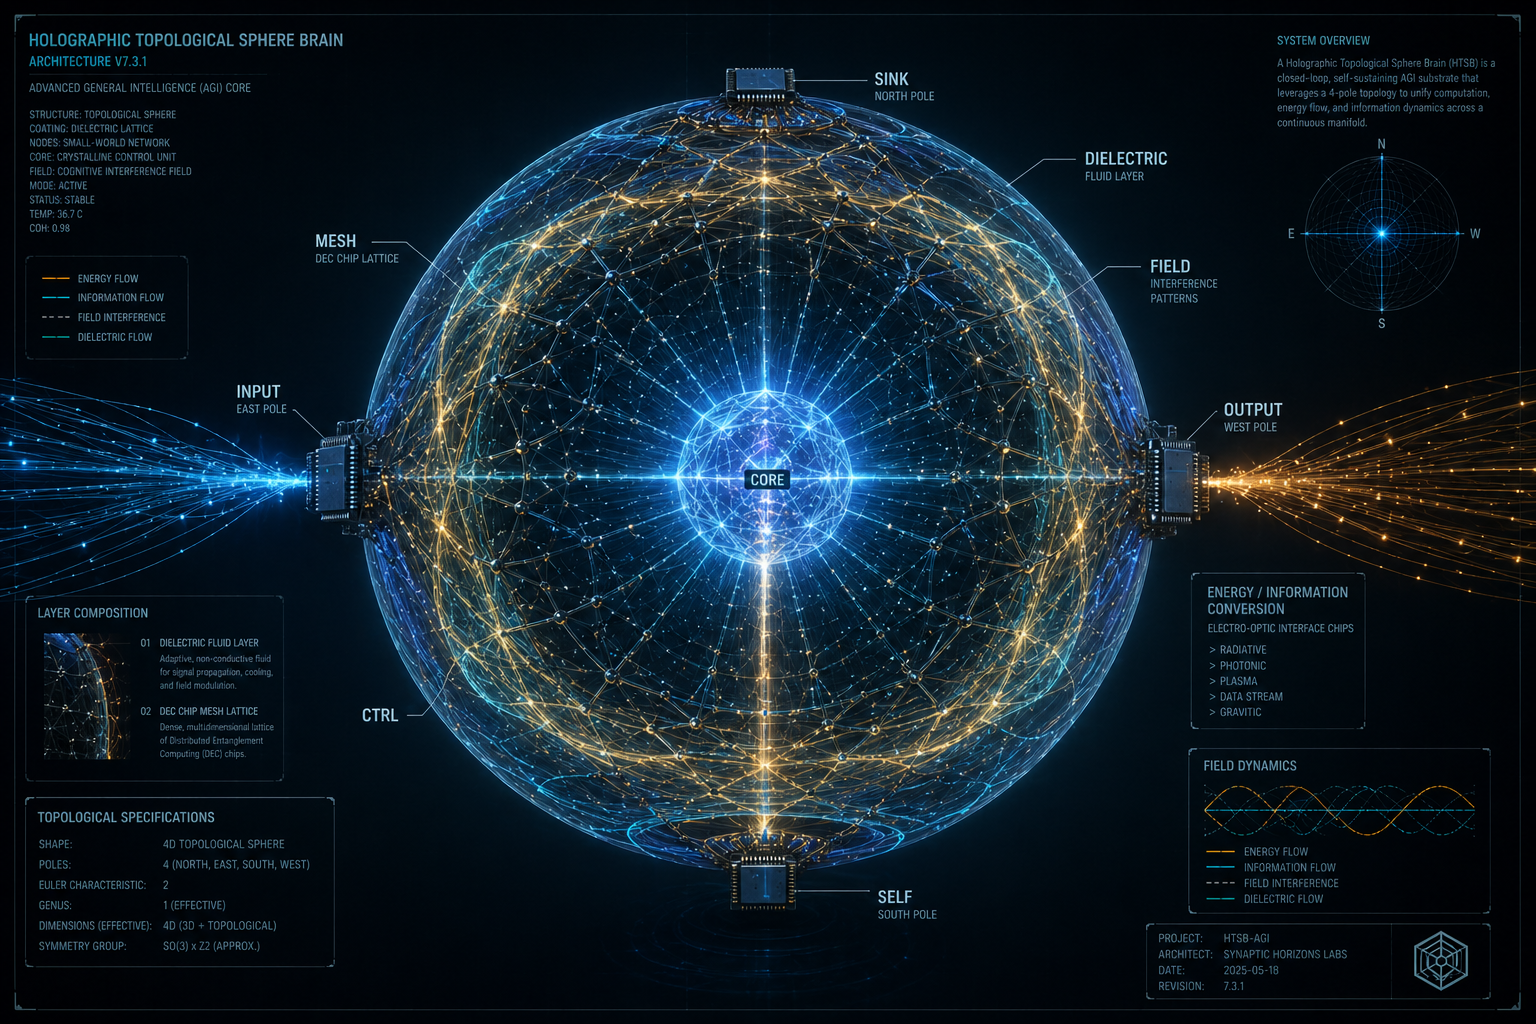
\includegraphics[width=0.9\textwidth]{image/dec.png}
\caption{DEC AGI芯片架构示意图}
\end{figure}
%---chp----
